\section{Zielsetzung}
In diesem Versuch soll die Halbwertszeit $T$ von Rhodium und Vanadium durch Beschuss stabiler Kerne mit Neutronen ermittelt werden.

\section{Theorie}
\label{sec:Theorie}
Sobald das Protonen und Neutronen Verhältnis außerhalb des Stabilitätsbereichs liegt, ist ein Atomkern instabil und zerfällt.
Nuklide zerfallen mit unterschiedlicher Wahrscheinlichkeit in einen stabilen oder in einen weiteren instabilen Kern, der wiederum zerfällt.
Durch die Halbwertszeit $T$ kann diese Zerfallswahrscheinlichkeit ausgedrückt werden.
In dieser Zeit zerfällt von einer großen Menge instabiler Kerne die Hälfte.
Da die hier zu ermittelnen Halbwertszeiten zwischen Sekunden und Stunden liegen, werden die Nuklide kurz vor Messbegin durch Beschießen von Kernen mit Neutronen hergstellt.

\subsection{Kernreaktion}
\label{subsec:Kernreaktion}
Kern A absorbiert ein Neutron, es ensteht ein Zwischenkern $A^*$.
Dieser ist um die Energie des Neutrons größer als Kern A.
Die Energie wird auf alle Nukleonen im Kern verteilt und erreichen dadurch höhere Energiezustände, auch Aufheizung des Zwischenkerns genannt.
Da die Energie gleich verteilt ist, ist eine Abstoßung eines Nukleons nicht möglich bzw. sehr unwahrscheinlich, besonders bei einfallenden Neutronen mit niedrieger Energie.
Durch Emission eines Photons nach ca. $\SI{e-16}{\second}$ erlangt der Kern A* wieder seinen Grundzustand.
Dieser neue Kern ist aber aufgrund der erhöhten Neutronenanzahl instabil.
Durch Aussendung des Photons verweilt er länger in diesem instabilen Zustand bis ein Elektron abgestoßen wird.
Dadurch geht dieser Kern in einen stabilenn Zustand über.
Die restliche Masse wandelt sich nach Einsteinschen Beziehung in kinetische Energie um.
\begin{align*}
    \ce{^{m}_{z}A -> ^{1}_0n -> ^{m{+1}}_{z}{A^{*}} -> ^{m{+1}}_{z}A + \gamma}\\
    \ce{^{m{+1}}_{z}A -> ^{m{+1}}_{z{+1}}C + \beta^{-} + E_{\text{kin}} + \overline{\nu}}
\end{align*}
\subsection{Wirkungsquerschnitt}
\label{subsec:Wirkungsquerschnitt}
Der Wirkungsquerschnitt $\sigma$ beschreibt die Fläche, die ein Kern haben müsste, um jedes Neutron einzufangen, das die Fläche trifft.
Er wird beschrieben durch:
\begin{equation*}
    \sigma =\frac{u}{nKd} ,
\end{equation*}
wobei D die Dicke , K die Atome [\si{\centi\meter}], n die Neutronen pro Sekunde und u die Einfänge ist.
Die Einheit von $\sigma$ ist $\SI{e-24}{\centi\metre\squared} = \SI{1}{\barn}$.
Dieser Querschnitt hängt stark von der Geschwindigkeit des Neutrons ab.

LOl do i need this. I DONT THINK SO .. ja eig nicht ne.
maybe wegen wenig geschwindigkeit?

\subsection{Erzeugung Niederenergetischer Neutronen}
\label{subsec:NeutronenHerstellen}
Niederenergetische Neutronen haben eine höhere Wahrscheinlichkeit vom Kern eingefangen zu werden.
Nun müssen diese erzeugt werden, da sie nicht natürlich vorkommen.
Das geschieht durch Kernreaktionen.
$\alpha$-Teilchen aus dem Zerfall von $\ce{^{226}Ra}$-Kernen werden auf $\ce{^{9}Be}$-Kerne geschossen um Neutronen zu erhalten.
Die durch den Beschuss entstandenen Neutronen können Energien von bis zu $\SI{13.7}{\mega\electronvolt}$ haben.
Deswegen werden sie mithilfe von elastischen Stößen abgebremst.
Hierzu sollen die Neutronen in eine dicke Materieschicht eindringen um durch die Stöße abgebremst zu werden.
Um eine effektive Abbremsung durchzuführen, soll die Masse der Neutronen und der Materieschicht so ähnlich wie möglich sein.
Der Mantel der Neutronenquelle besteht somit aus Paraffin (siehe Abbildung \ref{fig:QuelleQuerschnitt})
Nach mehreren Stößen zwischen einem Neutronen und den Paraffin-Protonen wird es zu einem sogenannten thermischen Neutron.
Seine Energie beträgt dann bei einer Temperatur $T = \SI{290}{\kelvin}$ etwa $\SI{0.025}{\electronvolt}$.

\begin{figure}
    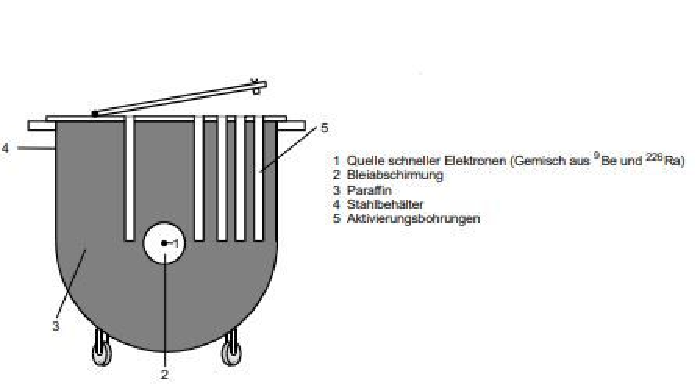
\includegraphics[width =\textwidth]{content/QuerschnittQuelle.pdf}
    \caption{Querschnitt der Neutronenquelle.\cite{anleitung}}
    \label{fig:QuelleQuerschnitt}
\end{figure}

\subsection{Untersuchung des Zerfalls instabiler Isotope}
Die Halbwertszeiten von Rhodium und Venedium sollen ermittelt werden.
Dazu werden Proben, die die Nuklide enthalten, in die Aktivierungsschächte der Neutronenquelle eingelegt.
Durch $\beta^-$-Zerfall gehen die instabilen Isotope in stabile über.
Zur Bestimmung der Halbwertszeit wird die Funktion des radioaktiven Zerfalls benötigt:
\begin{equation}\label{eqn:radioZerfall}
    N(t) = N_0 \symup{e} ^{-\lambda t} .
\end{equation}
Sie beschreibt die Anzahl der noch nicht zerfallenen Kerne zum Zeitpunkt $t$.
$N_0$ ist die Anzahl der instabilen Kerne zu Beginn der Messung.
$\lambda$ ist ein Ausdruck für die Zerfallswahrscheinlichkeit und wird Zerfallskonstante genannt.
Die Halbwertszeit $T$ kann dann mit der Gleichung \eqref{eqn:radioZerfall} beschrieben werden:
\begin{align}
    \frac{1}{2} N_0 & = N_0 \symup{e}^{-\lambda T} \\* \label{eqn:halbwertszeit}
    \implies T & = \frac{\ln(2)}{\lambda} 
\end{align}
Da sich $N(t)$ schwer ermitteln lässt, wird $N_{\Delta t}(t)$ eingeführt.
$N_{\Delta t}(t)$ beschreibt die zerfallenen Kerne in einem festen Zeitintervall $\Delta t$.
Es gilt:
\begin{equation*}
    N_{\Delta t}(t) = N(t) - N(t + \Delta t)
\end{equation*}
und mit Gleichung \eqref{eqn:radioZerfall} folgt:
\begin{align*}
    N_{\Delta t}(t) & = N_0 (1 - \symup{e}^{-\lambda\Delta t}) \symup{e}^{-\lambda t}\\
    \iff \ln(N_{\Delta t}(t)) & = -\lambda t \ln(N_0(1 - \symup{e}^{-\lambda\Delta t}))
\end{align*}
Bei den Messungen ist auf die Wahl $\Delta t $ zu achten.
Wird $\Delta t $ zu klein gewählt, entstehen statistische Fehler für $N_{\Delta t}(t)$.
Bei zu großen $\Delta t$ kommen systematische Fehler bei $\lambda$ auf.\\
\\
Zusätzlich weist Rhodium eine Besonderheit auf.
Wird Rhodium aus 100\% Isotop $\ce{^{103}Rh}$ aktiviert, geht dieser mit 90\% Wahrscheinlichkeit in das instabile Isotop $\ce{^{104}Rh}$ über.
Mit 10\% Wahrscheinlichkeit entsteht das instabile Isotop $\ce{^{104i}Rh}$, das ein $\gamma$-Quant aussendet und dann in $\ce{^{104}Rh}$ übergeht.
Diese Zerfälle laufen parallel mit unterschiedlichen Halbwertszeiten ab.
\subsection{Messapparatur}
In der Abbildung \ref{fig:AufbauSkizze} ist der Aufbau der Messapparatur zu sehen.
Mithilfe eines Geiger-Müller-Zählrohrs können die ausgesondeten $\beta$- und $\gamma$-Teilchen nachgewiesen werden.
Um den Nulleffekt zu verringern befindet sich um das Zählrohr ein Abschirmblock aus Blei.
Sobald ein Teilchen registriert wird, wird ein Impuls an ein elektronisches Zählwerk weitergeleitet.
Aufgrund der zwei Anzeigen wird die Messung nicht unterbrochen.
Nachdem die eingestellte Messzeit $\Delta t $ vorüber ist, wird innerhalb von $\SI{100}{\nano\second}$ die Anzeige gewechselt.
Vor dem Einlegen einer Probe kann der Nulleffekt $N_u$ durch Höhenstrahlung und natürliche Radioaktivität gemessen werden.
\begin{figure}
    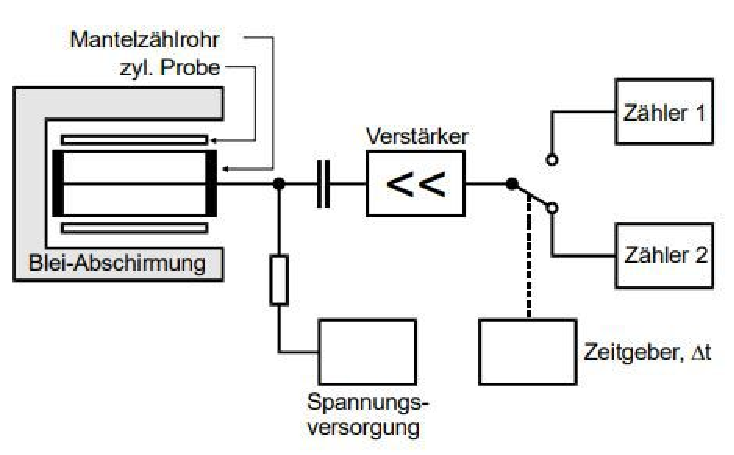
\includegraphics[width=\textwidth]{content/AufbauSkizze.pdf}
    \caption{Schematischer Versuchsaufbau.\cite{anleitung}}
    \label{fig:AufbauSkizze}
\end{figure}